%
% kubischer_ansatz.tex
%
% (c) 2024 Flurin Brechbühler
%
\begin{figure}
    \centering
    \subfloat[Formfunktionen des kubischen Ansatzes]{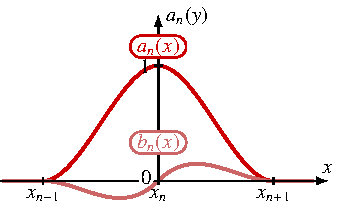
\includegraphics{papers/fem/images/kubisch_formfkt.pdf}\label{fem:1d:abb:kubisch:formfkt}}
    \hfill
    \subfloat[Skalierte Formfunktionen mit der zu interpolierenden Funktion $f(x)$]{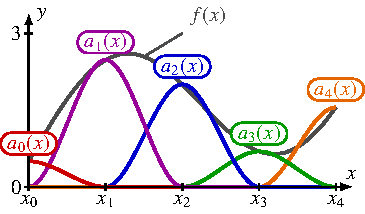
\includegraphics{papers/fem/images/kubisch_formfkt_skaliert.pdf}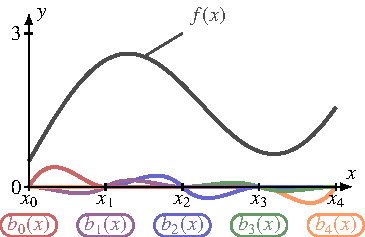
\includegraphics{papers/fem/images/kubisch_formfkt_skaliert_diff}\label{fem:1d:abb:kubisch:skaliert}}

    \subfloat[Gegenüberstellung der interpolierten und der uhrsprünglichen Funktion.]{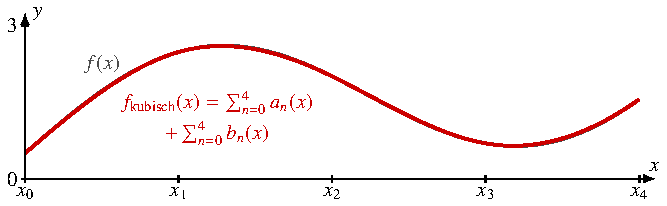
\includegraphics{papers/fem/images/kubisch_interpoliert.pdf}\label{fem:1d:abb:kubisch:vergleich}}
    \caption{Kubische Interpolation des Signals $f(x)$.}
    \label{fem:1d:abb:kubisch}
\end{figure}
    